%%%%%%%%%%%%%%%%%%%%%%%%%%%%
% CHAPTER                  %
%%%%%%%%%%%%%%%%%%%%%%%%%%%%

\section{Présentation de l'Agence Monégasque\\de Sécurité Numérique\\}
\label{chap1:section1}
{\fontsize{14pt}{16pt}\selectfont
    %%%%%%%%%%%%%%%%%%%%%%%%%%%%
% SECTION                  %
%%%%%%%%%%%%%%%%%%%%%%%%%%%%

L’Agence Monégasque de Sécurité Numérique (AMSN)\footnote{Site officiel de l’Agence Monégasque de Sécurité Numérique : \url{https://amsn.gouv.mc/}}, créée par Ordonnance Souveraine le 23 décembre 2015\footnote{\href{https://journaldemonaco.gouv.mc/Journaux/2015/Journal-8257/Ordonnance-Souveraine-n-5.664-du-23-decembre-2015-creant-l-Agence-Monegasque-de-Securite-Numerique}{Ordonnance Souveraine n° 5.664 du 23 décembre 2015}}, est l’autorité nationale en charge de la sécurité des systèmes d’information. Fondée sur le modèle de l'Agence Nationale de la Sécurité des Systèmes d'Information (ANSSI)\footnote{Site officiel du CERT-FR : \url{https://www.cert.ssi.gouv.fr/}} française, l'Agence est sous l’autorité directe du Ministre d’État (équivalent du Premier ministre français) et a pour rôle de constituer un centre d’expertise, de réponse et de traitement en matière de sécurité et d’attaques numériques pour l’Etat et les Opérateurs d’Importance Vitale (OIV) monégasques.\\

\vspace{1em}

L'AMSN est aujourd'hui structurée autour de deux pôles, exposés ci-après.

\newpage

\subsection{Le Pôle Expertise }

\vspace{1em}

Le Pôle Expertise forme un groupe d'experts qui joue un rôle crucial dans la conception, la mise en œuvre et le suivi des stratégies de cybersécurité de l'État, ainsi que dans la sensibilisation et l'évaluation de la sécurité de l'infrastructure numérique nationale. Ses missions peuvent être résumées comme suit :\\

\begin{itemize}[itemsep=1em]
    \item[•] Conseiller et coordonner les travaux interministériels sur la sécurité des systèmes d'information.
    \item[•] Contrôler l'application des mesures de sécurité adoptées par le Gouvernement sur les systèmes d'information des administrations et des opérateurs publics ou privés.
    \item[•] Sensibiliser les services publics et les opérateurs publics et privés aux exigences en matière de sécurité numérique.
    \item[•] Évaluer et qualifier les acteurs et services de sécurité numérique de la Principauté.
    \item[•] Mise en place et maintenance du service national de certification électronique pour les services de l'État, de la Commune, ainsi que les personnes physiques ou morales autorisées.
\end{itemize}

\vspace{1em}

Dans le cadre de mon stage, il m'a parfois été donné l'occasion de côtoyer le Pôle Expertise. Ce qui m'a permis d'assister à certaines de leurs activités quotidiennes ainsi que de bénéficier de leur point de vue sur l'orientation de ma thèse.

\newpage

\subsection{Le Centre de réponse et de traitement en matière\\ d’attaques numériques (CERT-MC) }

\vspace{1em}

Afin d'être à même  de participer à la coopération internationale face aux menaces numériques, l'AMSN s'est dotée d'un CERT suivant les standards établis par le FIRST\footnote{\url{https://www.first.org}}, l'organisme qui coordonne l'action des différents CERTs et CSIRTs au niveau mondial.\\

Celui-ci réalise diverses missions réparties entre les trois divisions suivantes :\\

\begin{itemize}[itemsep=1em]
    \item[•] \textbf{La division en charge de la supervision et de la détection des événements de sécurité numérique ou « Security Operations Center » (SOC-MC)}\\
    Cette division est dédiée à la supervision et à la détection des événements de sécurité numérique. Sa mission principale est de protéger les systèmes d'information de la Principauté de Monaco contre les cybermenaces en temps réel, en assurant une vigilance constante et une réponse rapide aux évènements de sécurité. Une fois identifiés et analysés, ces évènements peuvent être déclarés comme incidents de sécurité lorsque leur dangerosité est avérée.
    \item[•] \textbf{La division en charge de la réponse aux incidents de sécurité numérique ou « Computer Security Incident Response Team » (CSIRT-MC)}\\
    Cette division a pour mission principale de répondre aux incidents de sécurité numérique (une fois ces derniers déclarés par le SOC-MC) en fournissant une assistance technique, des analyses approfondies et des solutions de remédiation aux parties prenantes (Étatiques et OIV publics ou privés) victimes.
    \item[•] \textbf{La division en charge de l’analyse, du partage et de l’information ou 
    « Information Sharing and Analysis Center » (ISAC-MC)}\\
    Cette division réalise la collecte, l'analyse et le partage d'informations liées à la cybersécurité provenant de diverses sources. Elle agit comme un centre névralgique pour la coordination des efforts de sécurité numérique, favorisant la collaboration entre les différents acteurs nationaux et internationaux.\\
\end{itemize}

Dans le cadre de mon stage, j'ai travaillé de façon concomitante au CSIRT-MC et au SOC-MC, sous la supervision de Bruno VALENTIN (mon tuteur de stage et responsable du CERT-MC) et de Sébastien ABBONDANZA (responsable du SOC-MC), car l'objectif de ma mission était d'améliorer certains processus de travail communs aux deux divisions. La suite de ce document se concentrera sur le CERT-MC; c'est auprès de ses équipes et avec son soutien que mon travail a été réalisé.
}

\newpage

\section{Problématique}
\label{chap1:section2}
{\fontsize{14pt}{16pt}\selectfont
    %%%%%%%%%%%%%%%%%%%%%%%%%%%%
% SECTION                  %
%%%%%%%%%%%%%%%%%%%%%%%%%%%%
\vspace{1em}

Sur le territoire de la Principauté, l'AMSN doit épauler la sécurité numérique de plusieurs dizaines d'administrations publiques et d'entreprises classées OIV, représentant autant de réseaux à superviser avec des milliers d'utilisateurs et d'appareils connectés.
L'Agence ne peut mener à bien cette mission qu'avec la coopération de ces acteurs, qui l'autorisent à placer des sondes en amont, et parfois à l'intérieur, de leurs réseaux. Toutes les actions des utilisateurs qui entrent et sortent des réseaux supervisés passent par les sondes qui disposent d'un IDS, en l'occurrence ici Suricata, lequel contrôle le contenu de ces flux réseau à l'aide de règles de détection qui, si elles sont déclenchées, génèrent des événements de sécurité gérés par le SOC-MC.

\begin{figure}[h]%
    \center%
    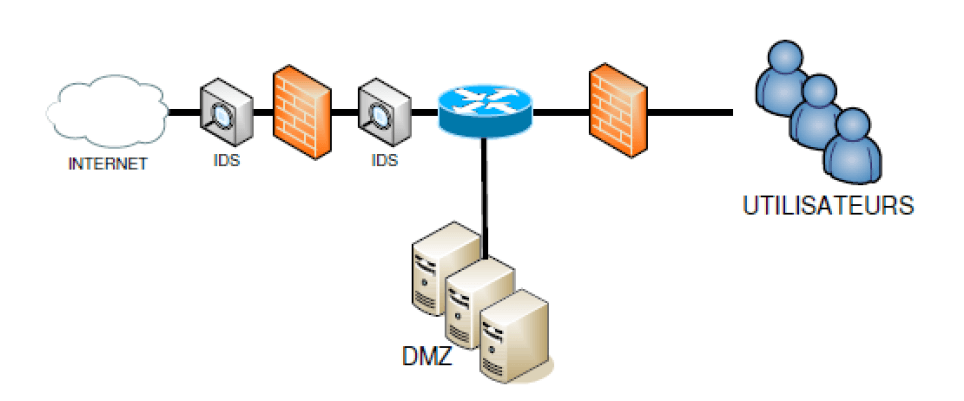
\includegraphics[width=1\textwidth]{assets/reseau.png}
    \caption[Exemple de disposition de sonde IDS dans le réseau d'un OIV (source:\href{https://blogger.googleusercontent.com/img/b/R29vZ2xl/AVvXsEhz0rffx8tqoJRqjF0Hf3LAERS8e7tpmQVnPzlBITzud8iMUOh63zfDIyLKLXnQprLLNAycblYb02W3Y4004q3ruHhdZ3T9Dy7KTMyydsLMRjR2UGkzQ6hIOcwM8DiSLeLp0pZeyyCt5CDl/s1600/Capture.PNG}{eventus-networks.blogspot.com})]{Exemple de disposition de sonde IDS dans le réseau d'un OIV}\label{fig:test}
\end{figure}

\vspace{1em}

Ces règles sont créées à partir d'indicateurs de compromission (IOC) établis en interne ou grâce à des renseignements externes provenant de CERT partenaires (comme le CERT-FR de l'ANSSI) ou d'agences privées de cyber-renseignement (également appelées CTI). Les règles générées par ces partenaires externes posent souvent des problèmes :\\

\begin{itemize}[itemsep=0.75em]
    \item[•] Les règles générées sont fréquemment génériques et mal adaptées, engendrant trop d'événements inutiles ou redondants dans le réseau où elles sont mises en œuvre (ces réseaux sont tous basés sur des technologies différentes).
    \item[•] Les renseignements extérieurs ne proviennent que d'une poignée d'acteurs, et l'agence ne peut être certaine de pouvoir détecter toutes les menaces existantes à l'état de l'art.\\
\end{itemize}

\newpage

Ces difficultés de l'AMSN sont communes aux institutions publiques et aux entreprises qui doivent remplir les mêmes missions. Cela légitime la problématique posée : "Comment mettre en place un outil automatisé de génération de règles de détection d’intrusion ?"\\

Pour aborder cette problématique, il faut se poser les questions suivantes :
\vspace{0.5em}
\begin{itemize}[itemsep=0.5em]
    \item[•] Où recueillir le cyber-renseignement nécessaire à l'établissement des IOC ? Et comment évaluer la qualité de ces renseignements ?
    \item[•] Comment générer des règles automatiquement à partir de ces IOC ?
    \item[•] Comment s'assurer que ces règles soient aussi pertinentes que possible pour la partie prenante supervisée ?\\
\end{itemize}

Mes travaux, menés dans le cadre de l'AMSN, visent à répondre à cette problématique et à fournir une solution capable de résoudre les problèmes posés à l'Agence ou à tout autre acteur similaire oeuvrant pour la protection des systèmes d'information.
}

\newpage

\section{Organisation du stage}
\label{chap1:section3}
{\fontsize{14pt}{16pt}\selectfont
    %%%%%%%%%%%%%%%%%%%%%%%%%%%%
% SECTION                  %
%%%%%%%%%%%%%%%%%%%%%%%%%%%%
\vspace{1em}

Le stage s'est déroulé du 1er avril au 30 septembre 2024. Pendant cette période, j'ai bénéficié d'un bureau au sein du SOC-MC avec un ordinateur personnel connecté à un réseau séparé sur lequel j'ai été libre de réaliser tous les développements nécessaires à la réalisation de mon projet. Cette configuration avait l'avantage de me permettre d'être proche des personnes impliquées dans l'outil sur lequel je travaillais, ainsi tout au long de mon stage j'ai pu disposer de l'expérience et des conseils, d'une part, des analystes SOC de l'AMSN et, d'autre part, de mon tuteur de stage Bruno VALENTIN, qui m'a partagé les connaissances et les avis du CSIRT.\\

Le stage s’est déroulé en trois parties distinctes :
\vspace{0.5em}
\begin{enumerate}[itemsep=0.5em]
    \item Apprentissage des technologies et du contexte
    \item Développement de la solution
    \item Rédaction de la thèse\\
\end{enumerate}

La première partie correspond à mon premier mois de stage, au cours duquel j'ai pris connaissance de mon environnement de travail et des missions de l'Agence, ainsi que des différents corps qui la composent. Au cours des semaines inaugurales de mon stage, j'ai dédié le plus clair de mon temps à suivre le travail quotidien de mes collègues pour appréhender les outils qu'ils utilisaient et comprendre comment ils fonctionnaient.\\

Après cette phase d'apprentissage, j'ai pu commencer à développer la solution relative à 
la problématique visée. Cette phase a duré quatre mois, à l'issue desquels j'ai soumis la solution et la documentation à mon tuteur. Mon tuteur s'est chargé quant à lui de la mise en production de mon travail pendant le mois qui a suivi.\\

Le dernier mois de stage et jusqu'à son terme, ayant finalisé la mission qui m'avait été confiée par mon tuteur, j'ai pu me concentrer avec son appui à parfaire, au sein de l'agence, la rédaction de la présente thèse, en l'étoffant par des échanges constructifs.\\

Tout au long de ces périodes, Bruno VALENTIN et Sébastien ABBONDANZA ont suivi mon travail en programmant des rapports bimensuels au cours desquels j'ai régulièrement fait état de mes progrès et reçu des conseils de leur part.
}

%L'ajout d'une url~\url{www.google.fr}\\
%L'ajout d'une référence~\cite{web001}\\
%Ajout d'une image~\ref{fig:test}\\

%  \begin{figure}[h]%
%    \center%
%    \includegraphics[width=0.3\textwidth]{assets/logonoir.png}
%    \caption[Image de réference]{Test Image}\label{fig:test}
%  \end{figure}


%\begin{table}\begin{center}
%\begin{tabular}{c|c}
%Entrée & Sortie \\ \hline
%A & B \\
%C & D
%\end{tabular}
%\caption{Test Table}\end{center}
%\end{table}

%This is a second subsection\cite{gen1972}, \cite{schaeffer99}. ~\\

%   \begin{description}\addtolength{\itemsep}{-0.35\baselineskip}%
%     \item[\textbullet~\bfseries Menu Item] \hfill \\%
%       Menu Description.~\\%
%       {\textbf{Focus topics:~}\emph{Topic one, topic two, topic three, ...}}%
%     %
%     \item[\textbullet~\bfseries Menu Item] \hfill \\%
%       Menu Description.~\\%
%       {\textbf{Focus topics:~}\emph{Topic one, topic two, topic three, ...}}%
%     %
%     \item[\textbullet~\bfseries Menu Item] \hfill \\%
%       Menu Description.~\\%
%       {\textbf{Focus topics:~}\emph{Topic one, topic two, topic three, ...}}%
%   \end{description}

%   Also bullets such as:%
%   \begin{itemize}\addtolength{\itemsep}{-0.35\baselineskip}%
%     \item One%
%     \item Two%
%     \item Three%
%     \item Four%
%     \item \ldots%
%   \end{itemize}%
%   %

% \begin{equation} \label{eq:1}
% \sum_{i=0}^{\infty} a_i x^i
% \end{equation}

% The equation \ref{eq:1} is a typical power series.